\chapter{System Workflow} \label{system_workflow}

This section will present the workflow of the system. As previously mentioned, the next step was to expand the defined DSL, and to use attributes as a form of calculation. Furthermore, most of the productions were expandable, allowing for certain calculations to be injected over the tree.

With the grammar divided into 3 main parts (STRUCTURE, ERRORS, INPUT), different types of calculations occur at different sections. The STRUCTURE and ERRORS blocks are written in a single file (by the teacher) which is then joined with the INPUT block (written by the student). The process starts with searching for the teacher and student specification, and then compiling the meta-grammar. After that, a single file is passed on to the processor for verification. This is the file containing the three main parts.

Within the grammar itself, the first rule
\begin{figure}[h]
    \centering
    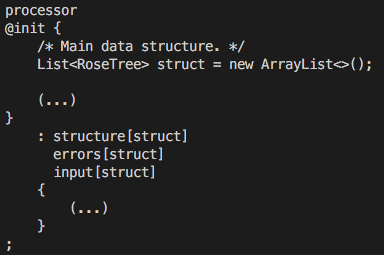
\includegraphics[width=8cm]{images/processor_expanded.png}
\end{figure}

\begin{lstlisting}[language=XML, caption= Concepts taught in the 1st year (fragment), label={lst:triplosAno1}]
    Triplos{
        ano1 =[
            desenvolve=> PensamentoComputacional,
            desenvolve=> RaciocinioLogico,
            desenvolve=> Abstraccao
        ];
    }
\end{lstlisting}

\noindent starts by initializing the main data structure. This structure is responsible for storing all the information that is being parsed from the file given as input (the meta-language file). It takes the form of a special tree, as each node may have numerous other nodes as children (\emph{Rose Tree}). The principle of having a tree as the main data structure falls into the need of maintaining a valid path. For example, if the teacher says that the structure will have a component \emph{\textbf{A}}, and this component has two children, \emph{\textbf{B}} and \emph{\textbf{C}}, then the paths \emph{\textbf{A$\rightarrow$B}} and \emph{\textbf{A$\rightarrow$C}} should be stored. In this particular problem, it is required to have a tree with multiple children that within each node has a list of children with an arbitrary size of \emph{\textbf{N}}.

When in the main production, a list of \emph{Rose Trees} is initialized, with each tree of the list corresponding to the main components of the sentence. This structure would travel along the parsing tree, to first be populated with information and then serving as the main source of validation and checking.

On the first block (STRUCTURE) there are not many calculations happening within the productions. The main task is to simply validate the syntax and extract data to be stored in the \emph{Rose Tree}. For each node, it is stored the name of the component, if it is required to be declared or not, a group of attributes (could be non existing), a lexical part (if it is the case), and finally a list of nodes, referred as the children.

After the parsing of the structure, there are a list of conditions named ERRORS that need to be validated and converted into \emph{Java} syntax - this conversion would then be injected on the main rule of the generated grammar. These logical expressions are based on the attributes of each component and their relations. For example, if the teacher says that a component \emph{\textbf{A}} has an attribute named \emph{\textbf{a}}, and this attribute is required to have value \emph{\textbf{x}}, if the student assigns it a value of \emph{\textbf{z}}, then an error should appear. All these conditions can be combined with the logical operands ``AND'' or ``OR''. The way that is parsed is based on the path specified by the teacher when accessing the attribute. Using the example before, a component \emph{\textbf{A}} with a child \emph{\textbf{B}}, with \emph{\textbf{B}} having a attribute \emph{\textbf{x}}, in order to access it the syntax should be

\begin{description}
    \Large{A.B -\textgreater x}
\end{description}
as the full path is required. This is done in order to calculate the correct path and avoid ambiguity between attributes. Over the parsing of these rules, the path is being validated, and in case of any error, the user is notified.

Finally, the last block corresponds to the input that was written by the student. The goal is to validate the components that were defined, and matched them with the structure created by the teacher. Again, the RoseTree was used as a way to check if the student’s components and paths were valid. The task of the student was to ''parse`` his sentence and divide it by components, identifying the lexical segments. When parsing these segments, they are stored within a node of the \emph{Rose Tree}, to then be injected into the generated grammar. In the case of any error, the user is informed of where the error happened but also in which component. Furthermore, when parsing attributes and their respective values, if the student defines two attributes with the same name, but with different values, a warning is raised to inform the user that the value that was considered was the last one to be recognized. 

Having parsed the meta-language file, a generator is called by the main rule - the \emph{Rose Tree} is passed as an argument and then traversed in order to generate all the rules for the grammar. This grammar, after being generated, is used to create a processor in which the student's sentence will be used as input, creating a visual syntax tree of that same sentence.